\subsubsection{Panel de Tasa de crecimiento poblacional y Consumo de energ�a anual}

\textsc{\begin{figure}[H]
	\centering
	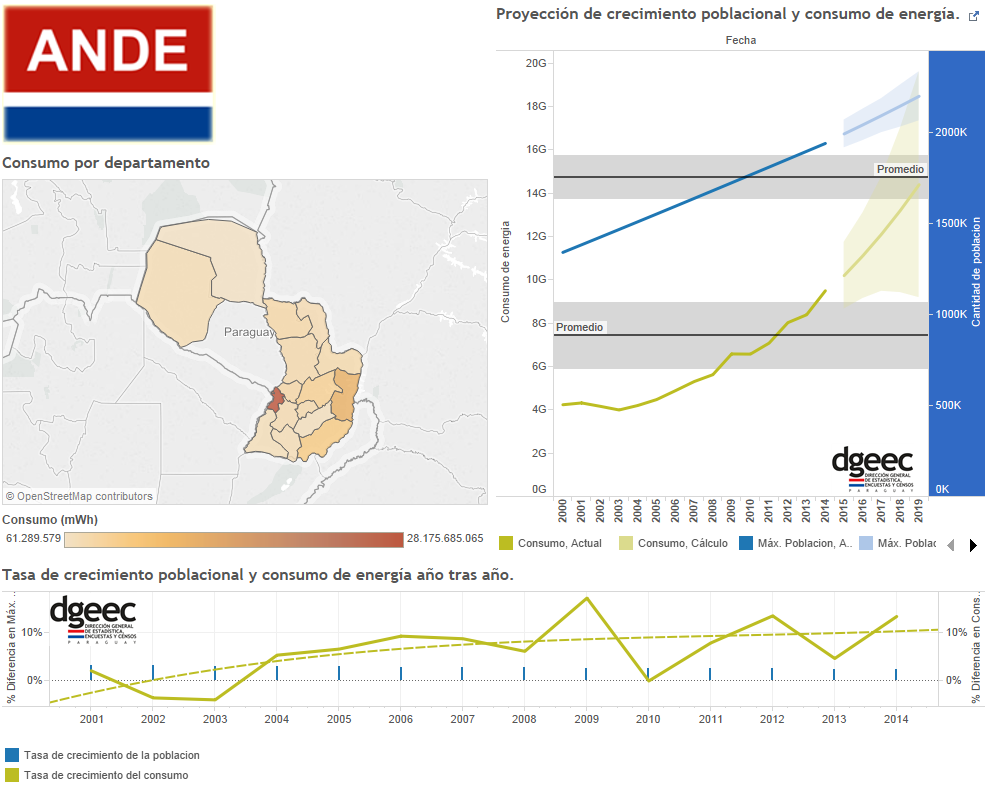
\includegraphics[width=\linewidth]{figuras/TasaDeCrecimientoPoblacionalYConsumoDeEnergiaAnoTrasAno}
	\caption{Panel de Tasa de crecimiento poblacional y Consumo de energ�a anual}
	\label{fig:TasaDeCrecimientoPoblacionalYConsumoDeEnergiaAnoTrasAno}
\end{figure}}

En la figura~\ref{fig:TasaDeCrecimientoPoblacionalYConsumoDeEnergiaAnoTrasAnoMapa} se presenta el panel comparativo de datos de crecimiento poblacional de la DGEEC y de consumo de la ANDE. En el mapa, cuando el color es m�s oscuro el consumo de energ�a es mayor, y si el color es m�s claro, el consumo es menor. Se puede notar que los departamentos Central y Alto Paran� son los que tiene mayor consumo de energ�a. 
Este tipo de gr�fico es muy �til cuando se desea analizar informaci�n de forma general y georeferenciada. Al ubicar el mouse sobre cualquier departamento, se presenta una ventana emergente indicando el valor de consumo del departamento seleccionado. Al seleccionar un departamento del mapa, los dem�s gr�ficos tambi�n se actualizan filtrando el departamento seleccionando. 

\textsc{\begin{figure}[H]
	\centering
	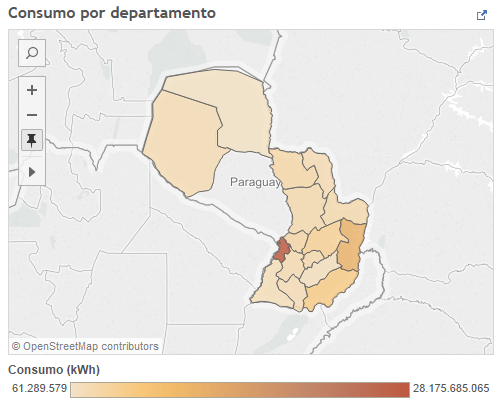
\includegraphics[width=\linewidth]{figuras/TasaDeCrecimientoPoblacionalYConsumoDeEnergiaAnoTrasAnoMapa}
	\caption{Consumo por departamento}
	\label{fig:TasaDeCrecimientoPoblacionalYConsumoDeEnergiaAnoTrasAnoMapa}
\end{figure}}
\noindent
 Los gr�ficos situados a la derecha y debajo del mapa presentan la tasa de crecimiento poblacional y de consumo de energ�a. Es importante notar que la tasa de crecimiento de la poblaci�n es casi constante, esto es, no tiene una gran variaci�n en el tiempo, ni una tendencia a alejarse de la media. Sin embargo, la tasa de crecimiento de consumo tiene una l�nea de tendencia a crecer durante el tiempo. As� puede apreciarse que, el consumo de energ�a no tiene una relaci�n de proporcionalidad con respecto al crecimiento de la poblaci�n.

\textsc{\begin{figure}[H]
	\centering
	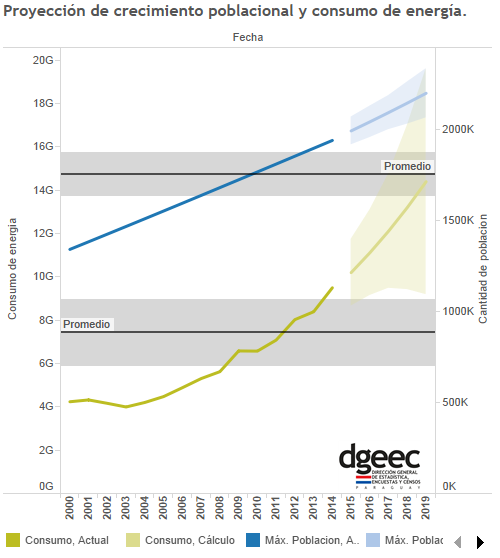
\includegraphics[width=\linewidth]{figuras/ProyeccionDeCrecimientoPoblacionalYConsumoDeEnergia}
	\caption{Proyecci�n de crecimiento poblacional y consumo ee energ�a}
	\label{fig:ProyeccionDeCrecimientoPoblacionalYConsumoDeEnergia}
\end{figure}}
\noindent
En este gr�fico,  se muestra la misma informaci�n que el gr�fico anterior pero con diferente perspectiva, en este caso se calcula el porcentaje de crecimiento anual tanto de la poblaci�n, as� como del consumo.


\textsc{\begin{figure}[H]
	\centering
	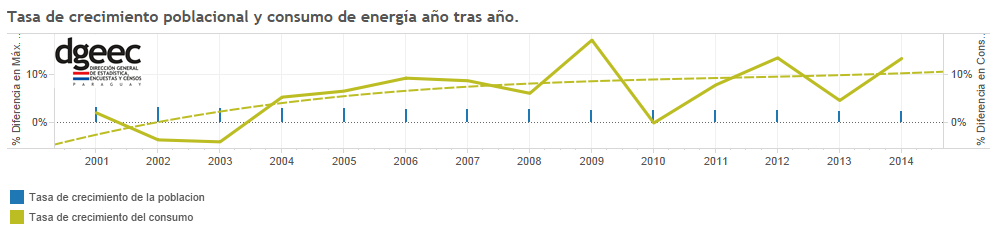
\includegraphics[width=\linewidth]{figuras/ProyeccionDeClientesYConsumosParaLosProximos5Anos2}
	\caption{Tasa de crecimiento poblacional y consumo de energ�a a�os tras a�os}
	\label{fig:ProyeccionDeClientesYConsumosParaLosProximos5Anos2}
\end{figure}}